\documentclass[12pt,a4paper]{article}

% ─── Page Layout ───────────────────────────────────────────────────────────────
\usepackage[a4paper, margin=0.8in, headheight=14pt]{geometry}

% ─── Fonts (XeLaTeX) ───────────────────────────────────────────────────────────
\usepackage{fontspec}
\usepackage{unicode-math}
\setmainfont{TeX Gyre Pagella}
\setmonofont[Scale=0.88]{TeX Gyre Cursor}
\setmathfont{Latin Modern Math}

% ─── Packages ──────────────────────────────────────────────────────────────────
\usepackage{xcolor}
\usepackage{colortbl}
\usepackage{titlesec}
\usepackage{enumitem}
\usepackage{tabularx}
\usepackage{booktabs}
\usepackage{array}
\usepackage{amsmath}
\usepackage{tikz}
\usetikzlibrary{shapes.geometric, arrows.meta, positioning, calc, fit, decorations.pathreplacing}
\usepackage{tcolorbox}
\tcbuselibrary{skins, breakable}
\usepackage{hyperref}
\usepackage{fancyhdr}
\usepackage{graphicx}
\usepackage{microtype}
\hyphenpenalty=10000
\exhyphenpenalty=10000
\sloppy
\usepackage{caption}
\usepackage{setspace}
\usepackage{multirow}
\usepackage{tocloft}

% ─── Q&A helper ────────────────────────────────────────────────────────────────
\newcommand{\Q}[1]{\textbf{#1}\par\noindent\ignorespaces}

% ─── Colour Palette ────────────────────────────────────────────────────────────
\definecolor{myred}{RGB}{196,30,58}
\definecolor{mydark}{RGB}{30,30,50}
\definecolor{mygreen}{RGB}{14,120,80}
\definecolor{myteal}{RGB}{0,130,140}
\definecolor{myamber}{RGB}{180,100,0}
\definecolor{mypurple}{RGB}{100,30,160}
\definecolor{mygray}{RGB}{246,247,249}
\definecolor{mgframe}{RGB}{180,185,200}
\definecolor{watermark}{RGB}{145,150,170}
\definecolor{hdrred}{RGB}{250,232,235}
\definecolor{hdrgreen}{RGB}{220,244,233}
\definecolor{hdrteal}{RGB}{220,242,244}
\definecolor{hdramber}{RGB}{253,242,215}
\definecolor{hdrpurple}{RGB}{238,228,255}
\definecolor{hdrgray}{RGB}{238,240,245}
\definecolor{rowalt}{RGB}{250,251,253}

% ─── Section Formatting ────────────────────────────────────────────────────────
\titleformat{\section}
  {\large\bfseries\color{myred}}{\thesection.}{0.5em}{}
  [\vspace{1pt}{\color{myred}\rule{\linewidth}{0.8pt}}]
\titleformat{\subsection}
  {\normalsize\bfseries\color{myteal}}{\thesubsection}{0.5em}{}
\titlespacing*{\section}{0pt}{18pt}{7pt}
\titlespacing*{\subsection}{0pt}{11pt}{4pt}

% ─── Paragraph ─────────────────────────────────────────────────────────────────
\setlength{\parindent}{0pt}
\setlength{\parskip}{4pt}

% ─── TOC Styling ───────────────────────────────────────────────────────────────
\renewcommand{\cfttoctitlefont}{\large\bfseries\color{myred}}
\renewcommand{\cftaftertoctitle}{\par\noindent{\color{myred}\rule{\linewidth}{0.8pt}}}
\setlength{\cftbeforetoctitleskip}{0pt}
\setlength{\cftaftertoctitleskip}{6pt}
\renewcommand{\cftsecfont}{\normalsize\bfseries\color{mydark}}
\renewcommand{\cftsecpagefont}{\normalsize\bfseries\color{mydark}}
\renewcommand{\cftsecleader}{\cftdotfill{\cftdotsep}}
\setlength{\cftbeforesecskip}{7pt}
\renewcommand{\cftsubsecfont}{\small\color{mydark}}
\renewcommand{\cftsubsecpagefont}{\small\color{mydark}}
\setlength{\cftbeforesubsecskip}{3pt}
\setlength{\cftsubsecindent}{1.4em}

% ─── Table helpers ─────────────────────────────────────────────────────────────
\renewcommand{\arraystretch}{1.45}
\setlength{\tabcolsep}{6pt}
\arrayrulecolor{mydark}
\newcolumntype{B}[1]{>{\small\bfseries\raggedright\arraybackslash}m{#1}}
\newcolumntype{Y}{>{\small\raggedright\arraybackslash}X}
\renewcommand{\tabularxcolumn}[1]{m{#1}}

% ─── Header / Footer ───────────────────────────────────────────────────────────
\pagestyle{fancy}
\fancyhf{}
\fancyhead[L]{\small\color{myred}\textbf{OE-EC704C}\;\color{mydark}--- Entrepreneurship}
\fancyhead[R]{\small\color{myteal}\textbf{Module 3 Notes}}
\fancyfoot[C]{\small\color{mydark}\thepage}
\fancyfoot[R]{\small\color{watermark}\textit{\copyright\ Biraj}}
\renewcommand{\headrulewidth}{0.5pt}
\renewcommand{\footrulewidth}{0.3pt}

% ─── Hyperref ──────────────────────────────────────────────────────────────────
\hypersetup{
  colorlinks=true, linkcolor=myteal, urlcolor=myteal,
  pdfauthor={Biraj Sarkar},
  pdftitle={OE-EC704C --- Module 3 Notes}
}

% ─── tcolorbox styles ──────────────────────────────────────────────────────────
\tcbset{
  tikzbox/.style={
    colback=mygray, colframe=mgframe, boxrule=0.6pt, arc=4pt,
    left=8pt, right=8pt, top=6pt, bottom=6pt,
    colbacktitle=mgframe, coltitle=mydark,
    fonttitle=\small\bfseries
  },
  defbox/.style={
    colback=hdrgreen, colframe=mygreen, boxrule=0.8pt, arc=4pt,
    left=9pt, right=9pt, top=6pt, bottom=6pt,
    colbacktitle=mygreen, coltitle=white,
    fonttitle=\small\bfseries
  },
  formulabox/.style={
    colback=hdrteal, colframe=myteal, boxrule=0.8pt, arc=4pt,
    left=9pt, right=9pt, top=7pt, bottom=7pt,
    colbacktitle=myteal, coltitle=white,
    fonttitle=\small\bfseries
  },
  examplebox/.style={
    colback=hdramber, colframe=myamber, boxrule=0.8pt, arc=4pt,
    left=9pt, right=9pt, top=6pt, bottom=6pt,
    colbacktitle=myamber, coltitle=white,
    fonttitle=\small\bfseries
  },
  masonbox/.style={
    colback=hdrpurple, colframe=mypurple, boxrule=0.8pt, arc=4pt,
    left=9pt, right=9pt, top=6pt, bottom=6pt,
    colbacktitle=mypurple, coltitle=white,
    fonttitle=\small\bfseries
  },
  exambox/.style={
    colback=hdrpurple, colframe=mypurple, boxrule=1pt, arc=5pt,
    left=10pt, right=10pt, top=8pt, bottom=8pt,
    colbacktitle=mypurple, coltitle=white,
    fonttitle=\bfseries,
    breakable, title after break={\textbf{Frequently Asked / Viva Questions (contd.)}}}
}
\tcbset{breakable}

% ─── TikZ styles ───────────────────────────────────────────────────────────────
\tikzset{
  block/.style={rectangle, draw=myteal, fill=hdrteal,
    text width=2.4cm, align=center, minimum height=0.95cm,
    font=\small, rounded corners=3pt, line width=0.7pt},
  redblock/.style={rectangle, draw=myred, fill=hdrred,
    text width=2.4cm, align=center, minimum height=0.95cm,
    font=\small, rounded corners=3pt, line width=0.7pt},
  netnode/.style={rectangle, draw=myteal, fill=hdrteal,
    text width=1.5cm, align=center, minimum height=0.8cm,
    font=\small, rounded corners=3pt, line width=0.7pt},
  sumjunc/.style={circle, draw=myamber, fill=hdramber,
    minimum size=0.62cm, font=\small, line width=0.8pt},
  snode/.style={circle, draw=mypurple, fill=hdrpurple,
    minimum size=0.55cm, font=\footnotesize, line width=0.7pt},
  arrow/.style={-Stealth, thick, color=mydark},
  redarrow/.style={-Stealth, thick, color=myred},
  line/.style={thick, color=mydark}
}

% ═══════════════════════════════════════════════════════════════════════════════
\begin{document}
% ═══════════════════════════════════════════════════════════════════════════════

\begin{center}
  {\LARGE\bfseries\color{myred} OE-EC704C --- Entrepreneurship}\\[5pt]
  {\normalsize\color{mydark} Semester VII \quad$\bullet$\quad 3L:0T:0P \quad$\bullet$\quad 3 Credits}\\[3pt]
  {\normalsize\color{myteal}\textbf{Module 3 Exam Notes: Financial Management, Accounting \& Taxation}}\\[3pt]
  {\small\color{mydark} CGEC \;$|$\; B.Tech ECE (2023--27) \;$|$\; \textit{Biraj Sarkar}}
\end{center}
\vspace{2pt}
\noindent{\color{myred}\rule{\linewidth}{1.5pt}}
\vspace{2pt}

\hypersetup{linkcolor=mydark}
\tableofcontents
\hypersetup{linkcolor=myteal}
\newpage

% ===============================================================================
\section{Financial Management \& Working Capital}
% ===============================================================================

\subsection{Financial Management Goals}
Financial management involves the planning, organizing, and controlling of financial resources to meet business objectives. There are two primary goals:
\begin{itemize}[leftmargin=*, itemsep=3.5pt]
  \item \textbf{Profit Maximization:} Focuses on increasing the net profit of the firm in the short term.
    \textit{Limitations:} Ignores the time value of money, ignores risks and uncertainty, and can lead to short-sighted decision-making.
  \item \textbf{Wealth Maximization (Value Maximization):} Focuses on maximizing the market value of the company's shares.
    \textit{Advantages:} Considers the time value of money, accounts for risk, and aims at long-term sustainable growth for shareholders.
\end{itemize}

\subsection{Working Capital Management}
Working capital represents the funds required to finance the day-to-day operations of an enterprise.

\begin{tcolorbox}[defbox, title={Working Capital Concepts}]
\begin{itemize}[leftmargin=*, itemsep=2.2pt, topsep=0pt]
  \item \textbf{Gross Working Capital:} Total investment in current assets (Cash + Receivables + Inventory + Short-Term Securities).
  \item \textbf{Net Working Capital:} Current Assets minus Current Liabilities. This represents the long-term funds financing current assets.
    \begin{equation}
      \text{NWC} = \text{Current Assets (CA)} - \text{Current Liabilities (CL)}
    \end{equation}
\end{itemize}
\end{tcolorbox}

\subsubsection{The Operating Cycle (Working Capital Cycle)}
The operating cycle is the duration of time required to convert raw materials back into cash through sales.

\begin{tcolorbox}[formulabox, title={Operating Cycle Length Calculation}]
The length of the Operating Cycle ($O$) in days is calculated as:
\begin{equation}
  O = R + W + F + D - C
\end{equation}
Where:
\begin{align*}
  R &= \text{Raw Material Storage Period} = \frac{\text{Average Stock of Raw Materials}}{\text{Daily Raw Material Consumption}} \\
  W &= \text{Work-in-Progress (WIP) Conversion Period} = \frac{\text{Average Stock of WIP}}{\text{Daily Cost of Production}} \\
  F &= \text{Finished Goods Storage Period} = \frac{\text{Average Stock of Finished Goods}}{\text{Daily Cost of Sales}} \\
  D &= \text{Debtors (Accounts Receivable) Collection Period} = \frac{\text{Average Accounts Receivable}}{\text{Daily Credit Sales}} \\
  C &= \text{Creditors (Accounts Payable) Payment Period} = \frac{\text{Average Accounts Payable}}{\text{Daily Credit Purchases}}
\end{align*}
\end{tcolorbox}

% ===============================================================================
\section{Costing and Book Keeping}
% ===============================================================================

\subsection{Elements of Cost}
Cost is divided into three primary categories to assist in pricing and control:
\begin{enumerate}[label=\textbf{\arabic*.}, leftmargin=*, itemsep=3pt]
  \item \textbf{Material Cost:} Cost of substances from which the product is manufactured.
    \begin{itemize}[label=\tiny$\bullet$, leftmargin=1.5em, itemsep=1.5pt]
      \item \textit{Direct Material:} Identifiable in the final product (e.g., steel in a car).
      \item \textit{Indirect Material:} Auxiliary items (e.g., lubricants, cleaning rags).
    \end{itemize}
  \item \textbf{Labour Cost:} Cost of wages paid to employees.
    \begin{itemize}[label=\tiny$\bullet$, leftmargin=1.5em, itemsep=1.5pt]
      \item \textit{Direct Labour:} Hands-on production staff (e.g., assembly line workers).
      \item \textit{Indirect Labour:} Supportive staff (e.g., supervisors, security).
    \end{itemize}
  \item \textbf{Expenses:} Cost of services other than materials and labor.
    \begin{itemize}[label=\tiny$\bullet$, leftmargin=1.5em, itemsep=1.5pt]
      \item \textit{Direct Expenses:} Hire charges for special tools for a specific job.
      \item \textit{Indirect Expenses (Overheads):} Rent, power, insurance, depreciation.
    \end{itemize}
\end{enumerate}

\subsection{Book Keeping Systems}
Bookkeeping is the recording phase of financial accounting.
\begin{itemize}[leftmargin=*, itemsep=3.5pt]
  \item \textbf{Single-Entry System:} An incomplete, informal system where only personal accounts and cash book records are maintained. It is prone to errors and cannot generate a balance sheet.
  \item \textbf{Double-Entry System:} A scientific, comprehensive system where every transaction affects at least two accounts (one debit, one credit) in opposite directions:
    \begin{equation}
      \text{Assets} = \text{Liabilities} + \text{Owner's Equity}
    \end{equation}
\end{itemize}

\subsubsection{Double-Entry Golden Rules of Accounting}
\par\noindent
{\renewcommand{\arraystretch}{1.5}%
\begin{tabularx}{\linewidth}{|B{3.0cm}|Y|Y|}\hline
\multicolumn{1}{|>{\centering\arraybackslash}m{3.0cm}|}{\textbf{Account Type}} &
\multicolumn{1}{>{\centering\arraybackslash}Y|}{\textbf{Debit Rules (Dr.)}} &
\multicolumn{1}{>{\centering\arraybackslash}Y|}{\textbf{Credit Rules (Cr.)}} \\
\hline
Real Account (Assets) & Debit what comes in. & Credit what goes out. \\
\hline
Personal Account (People/Firms) & Debit the receiver. & Credit the giver. \\
\hline
Nominal Account (Expenses/Gains) & Debit all expenses and losses. & Credit all incomes and gains. \\
\hline
\end{tabularx}
}

\subsubsection{Accounting Process Flow}
$$\text{Source Documents} \rightarrow \text{Journal (Day Book)} \rightarrow \text{Ledger (T-Accounts)} \rightarrow \text{Trial Balance} \rightarrow \text{Final Accounts}$$

% ===============================================================================
\section{Break-Even Analysis}
% ===============================================================================

Break-even analysis is a financial tool used to determine the level of output or sales volume at which a business earns zero profit and suffers zero loss.

\subsection{Mathematical Derivation of BEP}
Let:
\begin{align*}
  S &= \text{Selling Price per Unit} \\
  V &= \text{Variable Cost per Unit} \\
  F &= \text{Total Fixed Cost} \\
  Q &= \text{Quantity of Units Sold} \\
  R &= \text{Total Sales Revenue} = S \times Q \\
  TC &= \text{Total Cost} = F + (V \times Q) \\
  P &= \text{Net Profit} = R - TC = (S \times Q) - [F + (V \times Q)]
\end{align*}
At the \textbf{Break-Even Point (BEP)}, Profit ($P$) is zero:
\begin{equation*}
  (S \times Q_{BEP}) - F - (V \times Q_{BEP}) = 0
\end{equation*}
\begin{equation*}
  Q_{BEP} (S - V) = F
\end{equation*}
\begin{equation}
  Q_{BEP} \text{ (in Units)} = \frac{F}{S - V} = \frac{\text{Fixed Cost}}{\text{Contribution per Unit}}
\end{equation}
To find the Break-Even Sales value ($S_{BEP}$ in Rupees):
\begin{equation}
  S_{BEP} \text{ (in Rs.)} = Q_{BEP} \times S = \frac{F \times S}{S - V} = \frac{F}{1 - \frac{V}{S}} = \frac{\text{Fixed Cost}}{\text{P/V Ratio}}
\end{equation}

\subsection{Profit-Volume (P/V) Ratio \& Margin of Safety}
\begin{tcolorbox}[formulabox, title={P/V Ratio and Margin of Safety Formulas}]
\begin{itemize}[leftmargin=*, itemsep=3.5pt, topsep=0pt]
  \item \textbf{P/V Ratio (Contribution Margin Ratio):}
    \begin{equation}
      \text{P/V Ratio} = \frac{\text{Contribution}}{\text{Sales}} = \frac{S - V}{S} = \frac{\text{Fixed Cost} + \text{Profit}}{\text{Sales}}
    \end{equation}
  \item \textbf{Margin of Safety (MoS):} The excess of actual/planned sales over the break-even sales. It represents the cushion against sales drop before incurring a loss.
    \begin{equation}
      \text{MoS (in Units)} = \text{Actual Sales (Units)} - Q_{BEP}
    \end{equation}
    \begin{equation}
      \text{MoS (in Rs.)} = \text{Actual Sales Value} - S_{BEP} = \frac{\text{Profit}}{\text{P/V Ratio}}
    \end{equation}
    \begin{equation}
      \text{MoS Percentage} = \frac{\text{Actual Sales} - \text{BEP Sales}}{\text{Actual Sales}} \times 100\%
    \end{equation}
\end{itemize}
\end{tcolorbox}

\subsection{The Break-Even Chart}
The graphical representation of cost, volume, and profit relationships:

\begin{tcolorbox}[tikzbox, title={The Break-Even Chart}]
\centering
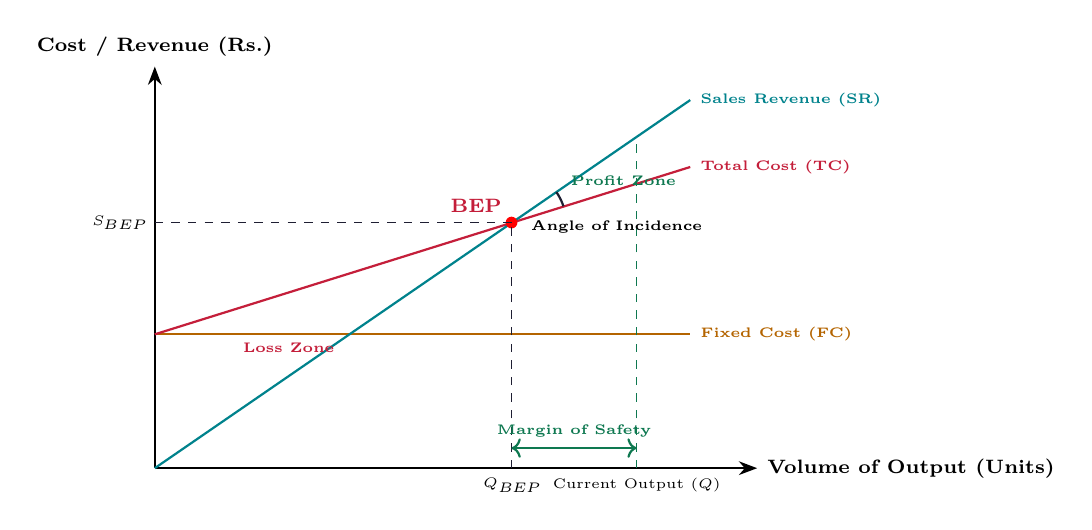
\begin{tikzpicture}[scale=0.85]
  % Draw Axes
  \draw[-Stealth, thick] (0,0) -- (9,0) node[right, font=\scriptsize\bfseries] {Volume of Output (Units)};
  \draw[-Stealth, thick] (0,0) -- (0,6) node[above, font=\scriptsize\bfseries] {Cost / Revenue (Rs.)};
  
  % Fixed Cost Line
  \draw[thick, color=myamber] (0,2) -- (8,2) node[right, font=\tiny\bfseries] {Fixed Cost (FC)};
  
  % Total Cost Line
  \draw[thick, color=myred] (0,2) -- (8,4.5) node[right, font=\tiny\bfseries] {Total Cost (TC)};
  
  % Sales Revenue Line
  \draw[thick, color=myteal] (0,0) -- (8,5.5) node[right, font=\tiny\bfseries] {Sales Revenue (SR)};
  
  % Break-Even Point Intersection
  % (5.5/8)*x = 2 + (2.5/8)*x => (3/8)*x = 2 => x = 16/3 = 5.33
  % y = (5.5/8)*5.33 = 3.67
  \coordinate (BEP) at (5.33,3.67);
  \fill[red] (BEP) circle (2.5pt);
  \node[above left, font=\scriptsize\bfseries, color=myred] at (BEP) {BEP};
  
  % Dashed projections from BEP
  \draw[dashed, color=mydark] (5.33,0) -- (5.33,3.67);
  \draw[dashed, color=mydark] (0,3.67) -- (5.33,3.67);
  \node[below, font=\tiny] at (5.33,0) {$Q_{BEP}$};
  \node[left, font=\tiny] at (0,3.67) {$S_{BEP}$};
  
  % Current output level projection
  \draw[dashed, color=mygreen] (7.2,0) -- (7.2,4.95);
  \node[below, font=\tiny] at (7.2,0) {Current Output ($Q$)};
  
  % Margin of Safety indicator
  \draw[<->, thick, color=mygreen] (5.33,0.3) -- (7.2,0.3) node[midway, above, font=\tiny\bfseries] {Margin of Safety};
  
  % Loss and Profit Zones
  \node[font=\tiny\bfseries, color=myred] at (2,1.8) {Loss Zone};
  \node[font=\tiny\bfseries, color=mygreen] at (7,4.3) {Profit Zone};
  
  % Angle of Incidence
  \draw[thick, color=mydark] (6.0,4.125) arc (35:18:0.8);
  \node[font=\tiny\bfseries] at (6.9,3.6) {Angle of Incidence};
\end{tikzpicture}
\end{tcolorbox}

% ===============================================================================
\section{Overview of Taxation}
% ===============================================================================

Taxes are compulsory levies by governments on individuals or corporations.

\subsection{Direct vs. Indirect Taxes}
\begin{itemize}[leftmargin=*, itemsep=3.5pt]
  \item \textbf{Direct Tax:} A tax levied directly on the income or wealth of a person or corporation (e.g., \textbf{Income Tax}). The burden of this tax cannot be shifted to another person.
  \item \textbf{Indirect Tax:} A tax levied on goods and services (e.g., \textbf{Excise Duty, Sales Tax, VAT, GST}). The burden is shifted to the final consumer in the form of higher prices.
\end{itemize}

\subsection{Traditional Indirect Tax Elements}
Before the implementation of GST (2017) in India, the indirect tax structure consisted of:
\begin{enumerate}[label=\textbf{\alph*.}, leftmargin=*, itemsep=2.5pt]
  \item \textbf{Excise Duty:} Tax levied on the manufacture/production of goods within the country.
  \item \textbf{Sales Tax:} Tax levied on the transfer of ownership of goods (intrastate or interstate).
  \item \textbf{Value Added Tax (VAT):} A multi-stage tax levied on the value added at each stage of production and distribution, allowing credit for tax paid on inputs (Input Tax Credit), which minimized cascading tax effects.
\end{enumerate}

\newpage

% ===============================================================================
% MANDATORY QUICK REVISION PAGE
% ===============================================================================
\begin{center}
  {\large\bfseries\color{myred} Quick Revision --- Module 3}\\[3pt]
  {\small\color{mydark} Accounting, BEP \& Taxation $|$ OE-EC704C}
\end{center}
\noindent{\color{myred}\rule{\linewidth}{1.2pt}}
\vspace{4pt}

\begin{tcolorbox}[formulabox, title={\textbf{Key Concepts \& Equations}}]
\renewcommand{\arraystretch}{1.4}
\begin{tabularx}{\linewidth}{B{4.0cm} X}
Net Working Capital & $\text{NWC} = \text{Current Assets} - \text{Current Liabilities}$. \\
Operating Cycle & $O = R + W + F + D - C$ (days). \\
BEP (Units) & $Q_{BEP} = \frac{\text{Fixed Cost}}{\text{Selling Price} - \text{Variable Cost}} = \frac{F}{S - V}$. \\
P/V Ratio & $\text{P/V} = \frac{\text{Contribution}}{\text{Sales}} = \frac{S - V}{S}$. \\
BEP (Rupees) & $S_{BEP} = \frac{\text{Fixed Cost}}{\text{P/V Ratio}}$. \\
Margin of Safety (MoS) & $\text{MoS (Rs.)} = \text{Actual Sales Value} - S_{BEP} = \frac{\text{Profit}}{\text{P/V Ratio}}$. \\
Accounting Equation & $\text{Assets} = \text{Liabilities} + \text{Capital}$. \\
\end{tabularx}
\end{tcolorbox}

\begin{tcolorbox}[defbox, title={\textbf{One-Line Definitions}}]
\begin{itemize}[leftmargin=*, itemsep=2.5pt, topsep=0pt]
  \item \textbf{Wealth Maximization:} Maximizing the long-term stock value of a company.
  \item \textbf{Operating Cycle:} Time taken from cash investment in raw materials to cash collection from buyers.
  \item \textbf{Nominal Accounts:} Accounts recording business expenses, losses, incomes, and gains.
  \item \textbf{Contribution:} Excess of sales revenue over variable costs ($S - V$).
  \item \textbf{Angle of Incidence:} The angle formed between the sales line and total cost line on a BEP chart; larger angles indicate faster profit generation.
  \item \textbf{Direct Tax:} Tax paid directly to the government by the earner (burden cannot be shifted).
  \item \textbf{VAT:} Multi-stage tax on goods where tax paid on inputs is credited.
\end{itemize}
\end{tcolorbox}

\begin{tcolorbox}[exambox, title={\textbf{Frequently Asked / Viva Questions}}]
\begin{enumerate}[topsep=0pt, label=\textbf{Q\arabic*.}, itemsep=5pt]
  \item \Q{Compare Profit Maximization and Wealth Maximization.}
    Profit Maximization is short-term and ignores risk and the time value of money. Wealth Maximization is a long-term goal that maximizes the market value of company shares, taking risk and timing of cash flows into account.
  \item \Q{What is the effect of increasing the credit period allowed to debtors on working capital?}
    Increasing the debtor credit period ($D$) lengthens the operating cycle, keeping capital tied up longer and increasing the working capital requirement.
  \item \Q{State the golden rule of real accounts.}
    Debit what comes in (increase in assets); Credit what goes out (decrease in assets).
  \item \Q{List the elements of cost in a manufacturing unit.}
    Cost of Materials (Direct and Indirect), Cost of Labour (Direct and Indirect), and Expenses/Overheads (Direct and Indirect).
  \item \Q{Differentiate between Journal and Ledger.}
    A journal is the book of prime entry where transactions are recorded chronologically. A ledger is the principal book where journal entries are classified and posted into individual accounts (T-accounts).
  \item \Q{What are the key assumptions in Break-Even Analysis?}
    Assumptions: All costs can be split into fixed and variable components; Fixed costs remain constant; Variable cost per unit remains constant; Selling price per unit remains constant; Sales volume equals production volume.
  \item \Q{What does a high Margin of Safety (MoS) indicate?}
    A high MoS indicates that the business is highly profitable and can withstand a significant decline in sales volume before hitting the break-even threshold and incurring losses.
  \item \Q{How does the Angle of Incidence affect profit capacity?}
    A large Angle of Incidence indicates a steep sales revenue line relative to total costs. It shows that the firm generates profits rapidly once the break-even point is passed.
  \item \Q{Differentiate between Direct and Indirect taxes with examples.}
    Direct tax (e.g., Income Tax) is levied on income and the burden cannot be shifted. Indirect tax (e.g., GST or Excise Duty) is levied on goods and services, and the cost burden is shifted to the final consumer.
  \item \Q{What is Input Tax Credit (ITC) under VAT?}
    ITC allows a manufacturer or seller to deduct the tax already paid on purchases (inputs) from the tax liability on sales (outputs), avoiding double taxation on the same product.
  \end{enumerate}
\end{tcolorbox}

\end{document}
